
\documentclass[a4paper,12pt]{article}

\usepackage{graphicx} % Required for inserting images
\usepackage{amsmath,amssymb,amsfonts}
\usepackage{subcaption}
% -----------------------
% Package Imports
% -----------------------

% Set page margins
\usepackage[a4paper, top=1in, bottom=0.8in, left=1.1in, right=0.8in]{geometry}

% Use Times New Roman font
\usepackage{times}

% Add page numbering
\pagestyle{plain}

% Enable graphics inclusion
\usepackage{graphicx}
\usepackage{float}
% Enable code listings
\usepackage{listings}
\usepackage{xcolor} % For customizing code colors
\setlength{\parindent}{0pt}




\begin{document}
	\section{Experiment No. 7}
	
	\section{Experiment Title }
Torque and Speed Characteristics of a DC Motor
	\section{Objective}
	
	The objectives of this lab are as follows:
	\begin{itemize}
	\item To investigate the torque and speed characteristics of a DC motor.
	\item To understand the relationship between torque and speed for DC motors.
	\item To observe the effect of varying load on the motor's speed and torque.
	\end{itemize}
	
	\section{Theory}
	
	\section*{Torque and Speed Characteristics of a DC Motor}
	 The performance of a DC motor is primarily evaluated based on its torque and speed characteristics, which determine its suitability for specific tasks. 
	

	
	Different types of DC motors, such as shunt and compound motors, exhibit unique torque and speed characteristics:
	\begin{itemize}
		\item \textbf{DC Shunt Motor:} Known for its excellent speed regulation, this motor maintains a nearly constant speed regardless of load variations.
		\item \textbf{DC Compound Motor:} Combines the properties of both shunt and series motors, offering higher starting torque and adjustable speed regulation, depending on the type of compounding.
	\end{itemize}
	\subsection{DC Shunt Motor}
	\subsubsection{$T / I_a$ Characteristics:}
	For a DC shunt motor, the torque (\(T\)) is directly proportional to the armature current (\(I_a\)). The torque equation is given by:
	
	\begin{equation}
		T = K I_a \Phi
	\end{equation}
	
	Where:
	\begin{itemize}
		\item \(T\) is the developed torque,
		\item \(K\) is a constant depending on motor construction,
		\item \(I_a\) is the armature current,
		\item \(\Phi\) is the flux per pole.
	\end{itemize}
	
	In a shunt motor, the field winding is connected in parallel with the armature winding. Since the supply voltage (\(V\)) is constant, the field current (\(I_f\)) remains nearly constant, and hence the flux (\(\Phi\)) is constant. Therefore, the torque equation simplifies to:
	
	\begin{equation}
		T \propto I_a
	\end{equation}
	
	This indicates that the torque varies linearly with the armature current. As a result, the torque characteristic of a DC shunt motor is represented by a straight line passing through the origin.
	\subsubsection{$Speed / I_a$ Characteristics:}
	The speed \( S \) of a DC shunt motor can be controlled by manipulating either the armature current \( I_a \) or the field flux \( \Phi \), as shown in the following formula:
	
	\[
	S = \frac{V_T - I_a R_a}{K \Phi}
	\]
	
	
	Where:
	\begin{itemize}
		\item \(S\) is the speed of the motor,
		\item \(V_T\) is the terminal voltage,
		\item \(I_a\) is the armature current,
		\item \(R_a\) is the armature resistance,
		\item \(K\) is a constant depending on motor construction,
		\item \(\Phi\) is the flux per pole.
	\end{itemize}
	
	In a DC shunt motor, the field winding is connected in parallel with the armature winding, which ensures that the flux (\(\Phi\)) remains constant under varying load conditions. As the load increases, the armature current (\(I_a\)) also increases, leading to a voltage drop across the armature resistance (\(I_a R_a\)). This reduces the back EMF, and consequently, the speed (\(S\)) decreases slightly.
	
	Since the flux remains constant, the speed reduction is minimal, resulting in good speed regulation. The speed characteristic curve for a DC shunt motor shows a slight deviation from a flat horizontal line, indicating relatively small speed changes with varying load conditions.
	
	\subsection{DC Compound Motor}
	\subsubsection{Cumulative Compound Motor}
		\subsubsection{$T / I_a$ Characteristics:}
		
		In a cumulative compound motor, the torque (\(T\)) is influenced by both the armature current (\(I_a\)) and the combined magnetic flux from the shunt and series field windings. The total flux (\(\Phi\)) is the sum of the flux due to the shunt field (\(\Phi_f\)) and the flux due to the series field (\(\Phi_s\)). The torque can be expressed as:
		
		\begin{equation}
			T = K I_a (\Phi_f + \Phi_s)
		\end{equation}
		
		
		Where:
		\begin{itemize}
			\item \(T\) is the developed torque,
			\item \(K\), \(K_1\), and \(K_2\) are motor-specific constants,
			\item \(I_a\) is the armature current,
			\item \(\Phi_f\) is the flux from the shunt field,
			\item \(\Phi_s\) is the flux from the series field.
		\end{itemize}
		
		As the load increases, the armature current (\(I_a\)) also increases. This causes the series field flux (\(\Phi_s\)) to increase, resulting in a more than linear increase in torque. This characteristic provides the motor with a "boost" in torque at higher loads, making cumulative compound motors well-suited for applications requiring high starting torque and improved load-handling capability.
		
		The torque characteristic curve of a cumulative compound motor shows a steeper rise compared to a shunt motor, especially at higher armature currents.
		
	
		
			\begin{figure}[H]
			\centering
			\begin{subfigure}[t]{.48\textwidth}
				\centering
					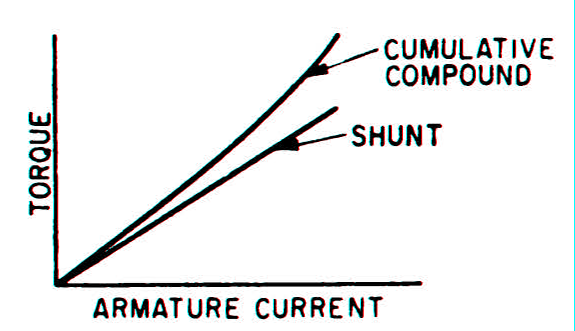
\includegraphics[width=1\linewidth]{Images/screenshot001}
				\caption{Comparing torque of cumulative and shunt motor}
				\vspace{0.5cm}
			\end{subfigure}
			\hfill
			\begin{subfigure}[t]{.48\textwidth}
				\centering
				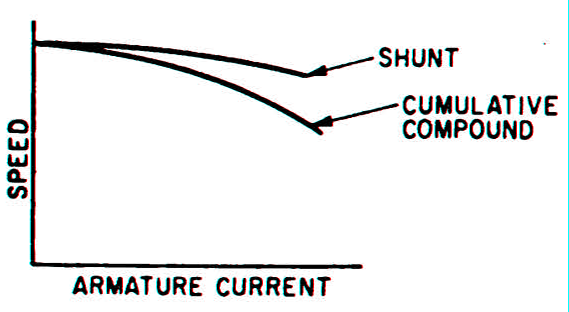
\includegraphics[width=1\linewidth]{Images/screenshot003}
			\caption{Comparing speed of cumulative and shunt motor}
			\end{subfigure}
			
			
		\end{figure}
		
			\subsubsection{$Speed / I_a$ Characteristics:}
			
			The speed (\(S\)) of a cumulative compound motor is influenced by the terminal voltage, armature current, resistances, and the combined flux from the shunt and series fields. It can be expressed as:
			
			\begin{equation}
				S = \frac{V_T - I_a (R_a + R_s)}{K (\Phi_f + \Phi_s)}
			\end{equation}
			
			Where:
			\begin{itemize}
				\item \(S\) is the speed of the motor,
				\item \(V_T\) is the terminal voltage,
				\item \(I_a\) is the armature current,
				\item \(R_a\) is the armature resistance,
				\item \(R_s\) is the series resistance,
				\item \(K\) is a motor-specific constant,
				\item \(\Phi_f\) is the flux due to the shunt field,
				\item \(\Phi_s\) is the flux due to the series field.
			\end{itemize}
			
			As the load on the motor increases, the armature current (\(I_a\)) also increases. This leads to a larger voltage drop across the combined resistance (\(R_a + R_s\)) and an increase in the series field flux (\(\Phi_s\)). Since the speed is inversely proportional to the total flux, the increase in \(\Phi_s\) causes the speed to decrease more rapidly compared to a shunt motor.
			
			The speed characteristic curve of a cumulative compound motor is less flat than that of a shunt motor. This means the motor experiences a more significant reduction in speed as the load increases, due to the cumulative effect of the series field. This characteristic makes cumulative compound motors suitable for applications where a decrease in speed with increasing load is acceptable or even beneficial.
			
			
			
			\subsubsection{Differential Compound Motor}
			\subsubsection{$T / I_a$ Characteristics:}
			
			In a differential compound motor, the torque (\(T\)) is influenced by both the shunt field flux (\(\Phi_f\)) and the series field flux (\(\Phi_s\)). However, unlike in a cumulative compound motor, the series field flux opposes the shunt field flux. The torque can be expressed as:
			
			\begin{equation}
				T = K I_a (\Phi_f - \Phi_s)
			\end{equation}
			
			
			
			Where:
			\begin{itemize}
				\item \(T\) is the developed torque,
				\item \(K\), \(K_1\), and \(K_2\) are constants depending on motor construction,
				\item \(I_a\) is the armature current,
				\item \(\Phi_f\) is the flux from the shunt field,
				\item \(\Phi_s\) is the flux from the series field.
			\end{itemize}
			
			As the load increases, the armature current (\(I_a\)) also increases, leading to a rise in the opposing series flux (\(\Phi_s\)). This reduces the net flux, which in turn decreases the torque at higher loads. 
			
			This characteristic makes differential compound motors unsuitable for heavy-load applications, as the torque decreases with increasing load, which can lead to instability and inefficient operation under such conditions.
			\subsubsection{$Speed / I_a$ Characteristics:}
	
	The speed (\(S\)) of a differential compound motor is influenced by the terminal voltage, armature current, resistances, and the net flux resulting from the opposing shunt and series fields. The speed equation is given by:
	
	\begin{equation}
		S = \frac{V_T - I_a (R_a + R_s)}{K (\Phi_f - \Phi_s)}
	\end{equation}
	
	
	
	In a differential compound motor, the series flux (\(\Phi_s\)) opposes the shunt flux (\(\Phi_f\)). As the load increases, the armature current (\(I_a\)) also increases, causing the opposing series flux (\(\Phi_s\)) to grow. This reduces the total flux (\(\Phi_f - \Phi_s\)).
	
	Since speed is inversely proportional to the net flux, the reduction in total flux causes the speed to increase as the load increases. This behavior is opposite to that of cumulative compound and shunt motors, where speed decreases with load.
	
	The speed characteristic curve of a differential compound motor thus shows an increase in speed with increasing load. This characteristic makes differential compound motors suitable for applications where a slight increase in speed under load is advantageous.
	
	
	\begin{figure}[H]
		\centering
		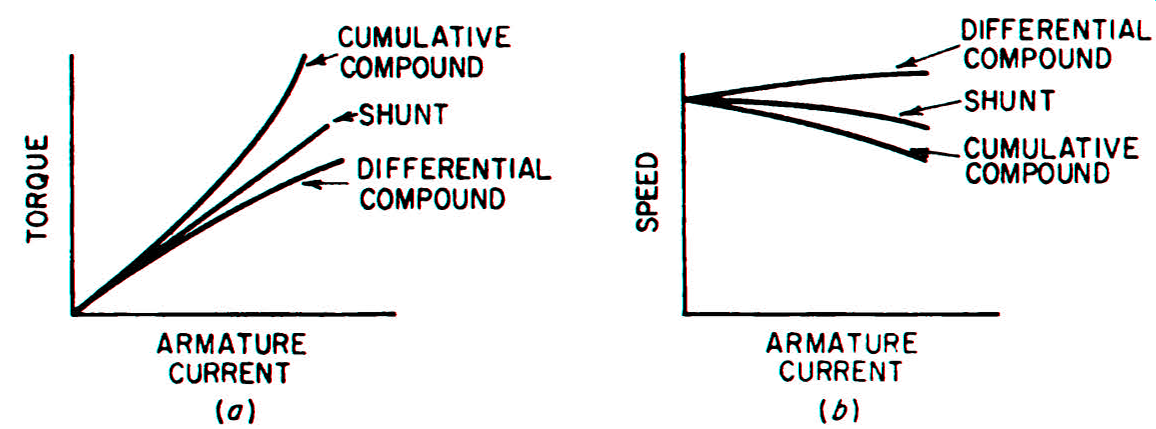
\includegraphics[width=0.89\linewidth]{Images/screenshot002}
		\caption{Comparison of Torque and Speed characteristics}
		\label{fig:screenshot002}
	\end{figure}
	
	
	
	
	
	
	\section{Required Apparatus}
	\begin{enumerate}
		\item Electric Machine Trainer
		\begin{enumerate}
			\item DC Motor Starting Resistor
		\item DC Power Supply (Rating: Voltage: 200V)
		\item DC Ammeters (Rating: Current: 5A)
		\item DC Voltmeter (Rating: Voltage: 500V)
		  \item DC Motor Field Resistor
		  	\item Speed Meter (Rating: 1500 rpm max)
		  \item Torque Meter (Rating: 0.24 kg-m max)
		\end{enumerate}
	  

	\item DC Compound Motor (Ratings: Output: 360W, Voltage: 200V, Current: 2.5A, Speed: 1500 rpm;  Field: 0.2A, Pole: 2P)
	\item Dynamometer (Ratings: Output: 360W, Voltage: 100V, Current: 3A; Pole: 2P; Speed: 4000 rpm max, Type: Eddy Current)

	\end{enumerate}
	\newpage
	\section{Circuit Diagrram}

	
	
	\begin{figure}[H]
		\centering
		\begin{subfigure}[t]{.9\textwidth}
			\centering
		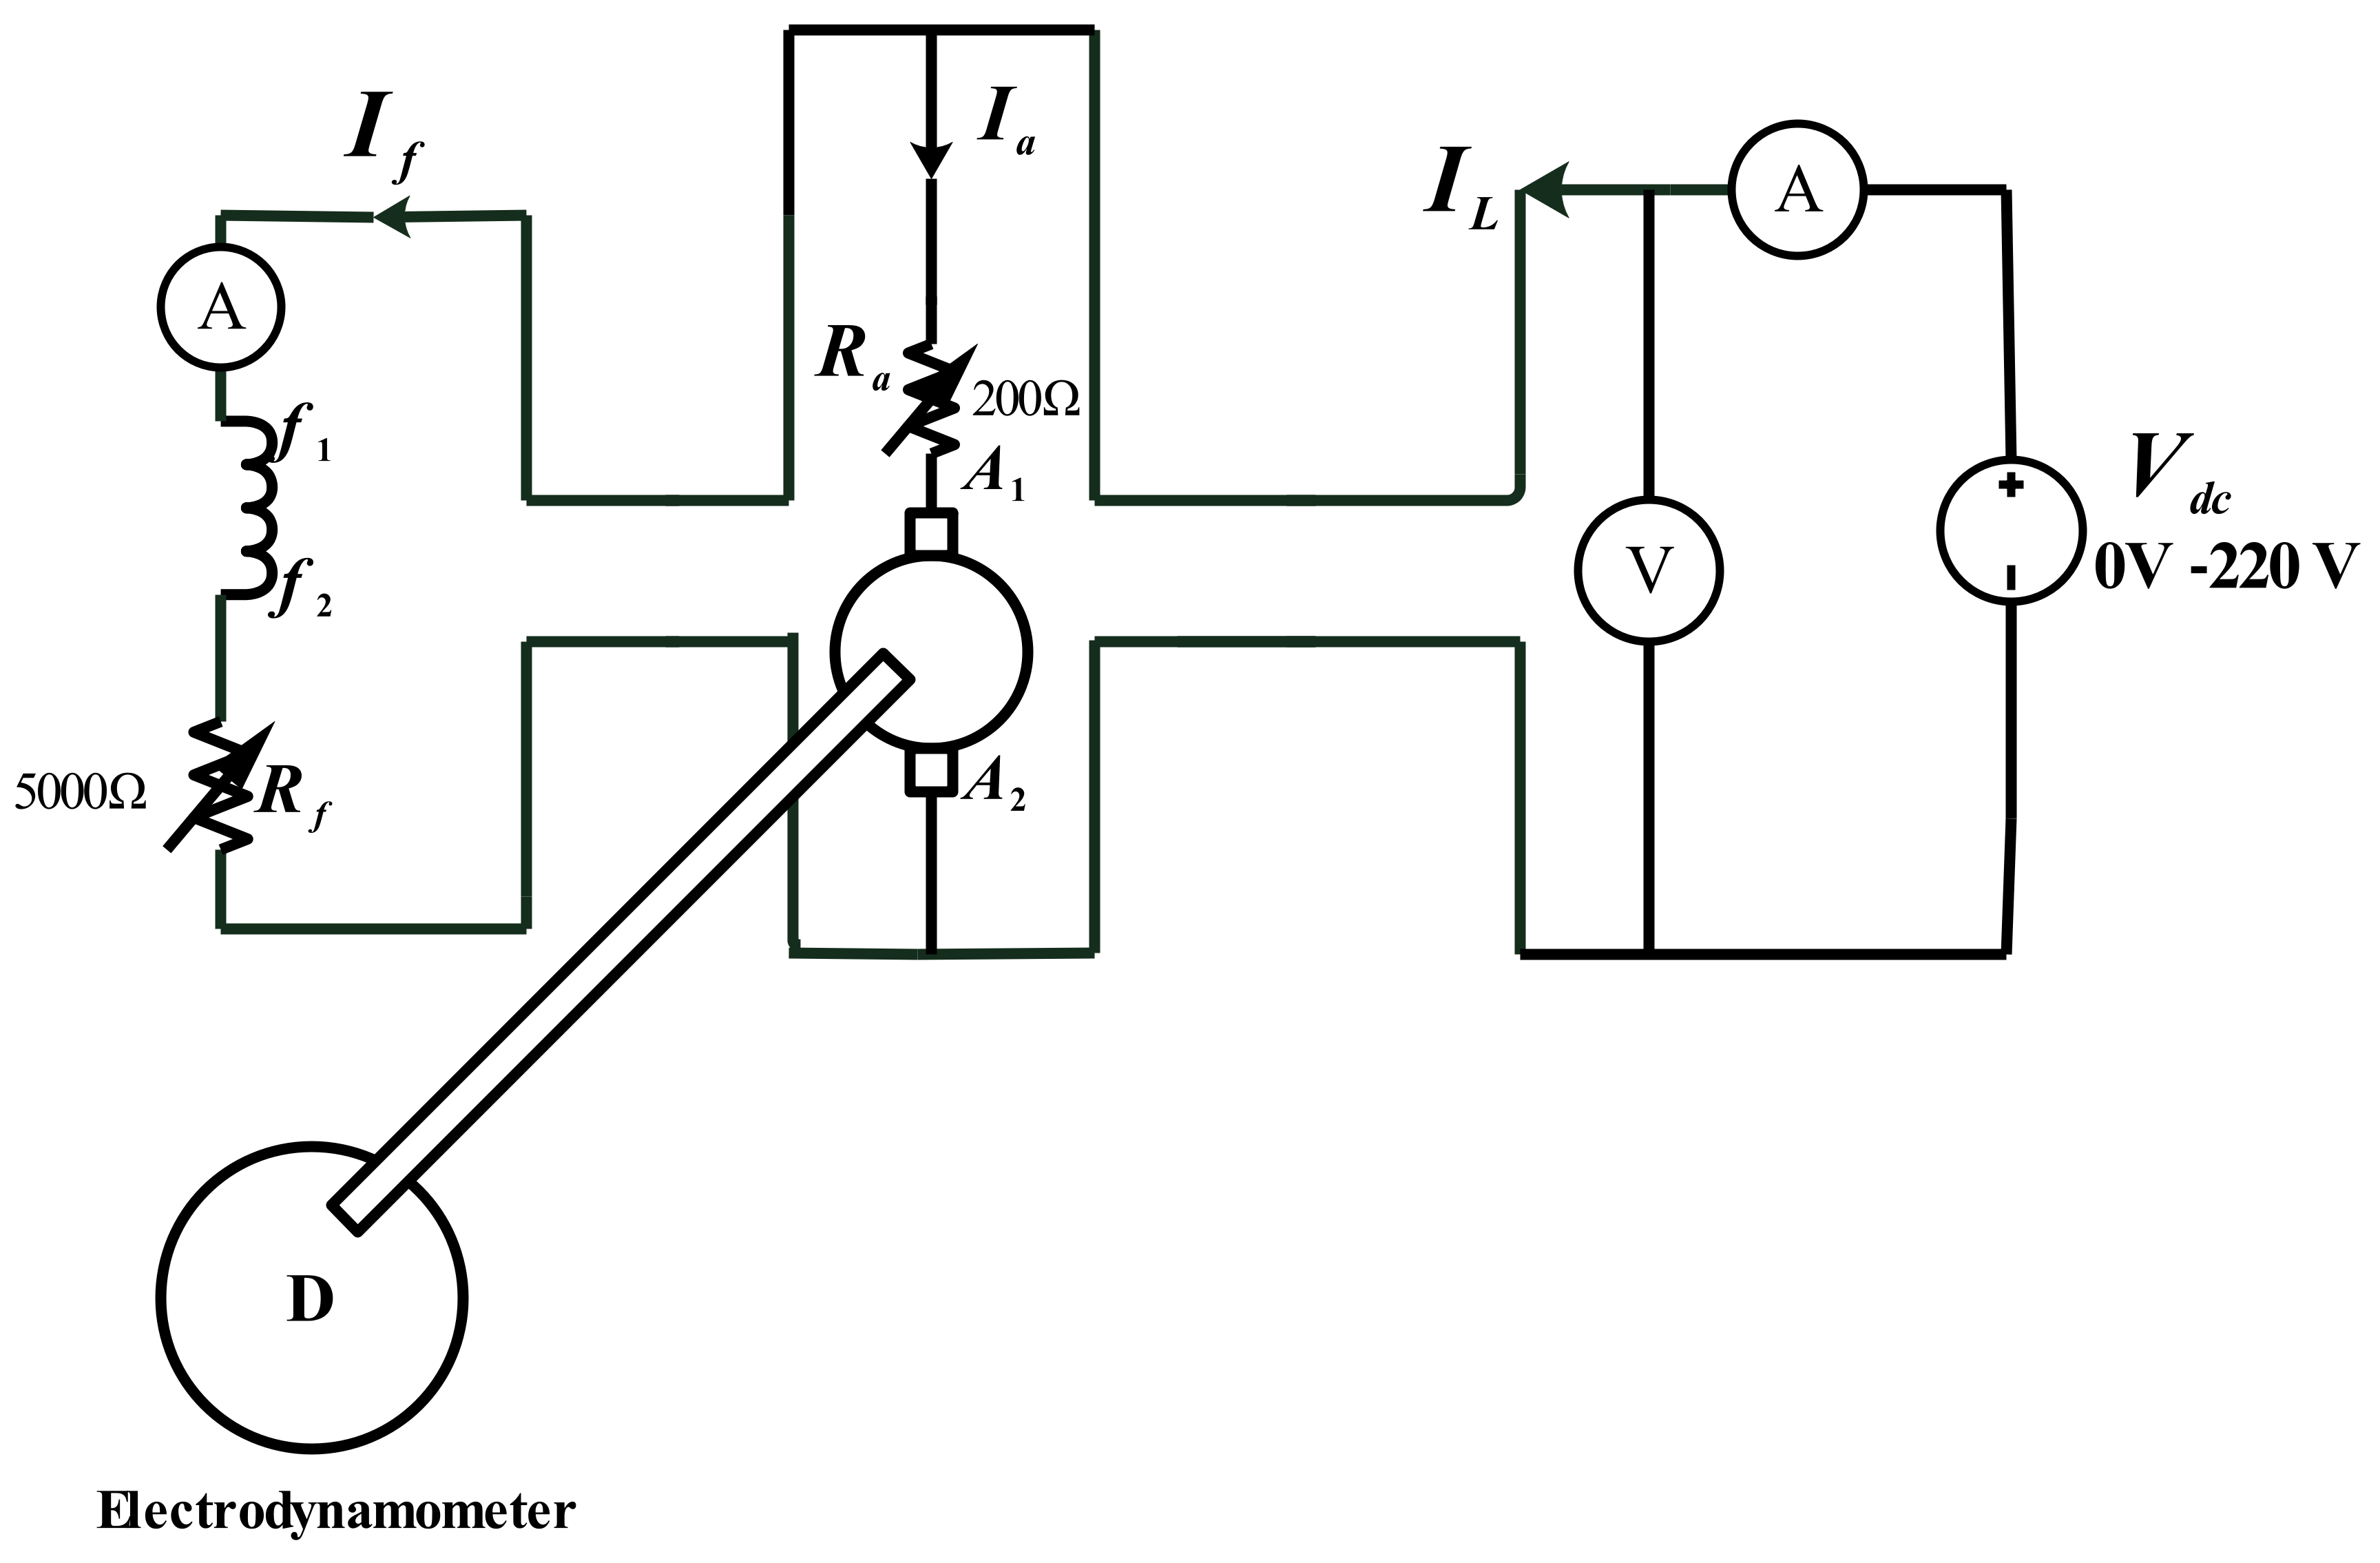
\includegraphics[width=1.1\textwidth]{Images/3.3}
			\caption{Circuit diagram for DC Shunt Motor}
			\vspace{0.5cm}
		\end{subfigure}
	
		\begin{subfigure}[t]{.9\textwidth}
			\centering
		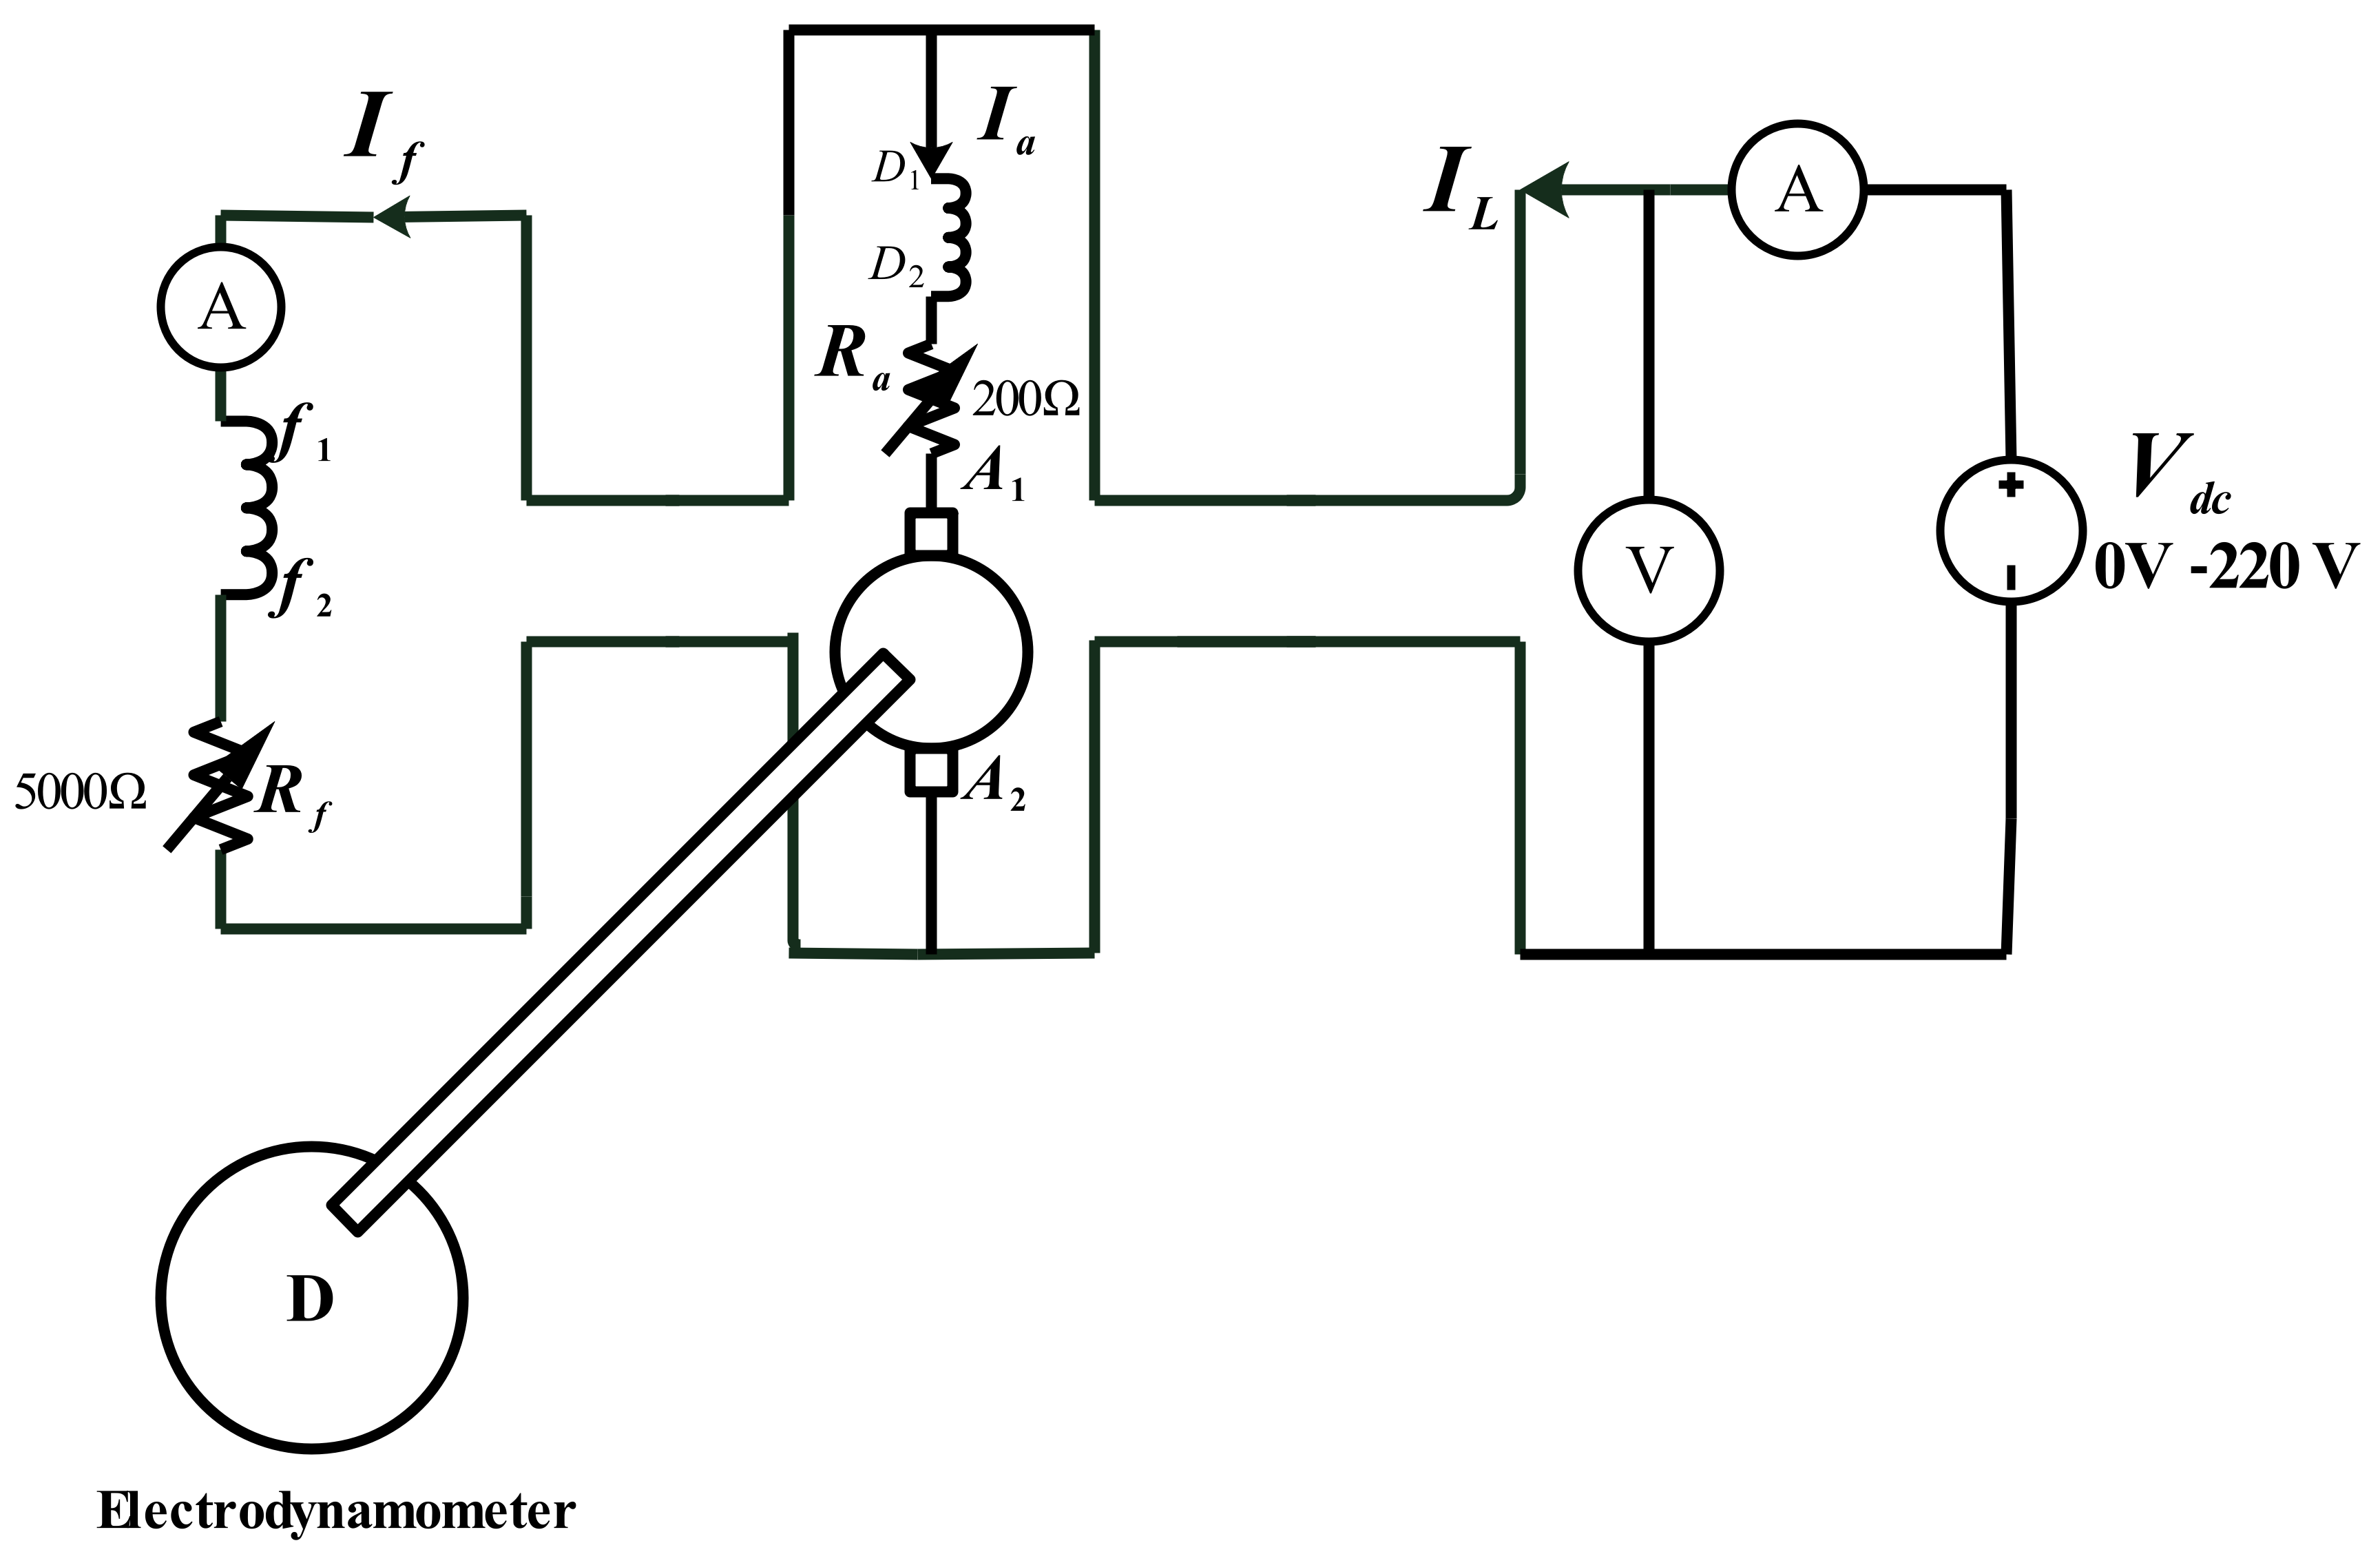
\includegraphics[width=1.1\textwidth]{Images/3.2}
			\caption{ Circuit diagram for DC Compound Motor }
		\end{subfigure}
		
		
	\end{figure}
	
	
	\newpage
	

	

	
	
		\section{Data Table}
	\begin{table}[H]
		\centering
		\caption{Readings of   Armature current $(I_a)$, Motor Speed $(S)$ and Torque($T$) }
		% Sub-table (a)
		\begin{subtable}[t]{0.45\textwidth} % Adjusted width for each sub-table
			\centering
			\begin{tabular}{|c|c|c|c|}
			\hline
			\textbf{\begin{tabular}[c]{@{}c@{}}SI   \\ No.\end{tabular}} & \textbf{\begin{tabular}[c]{@{}c@{}}Armature\\ Current,\\ $I_a (A) $\end{tabular}} & \textbf{\begin{tabular}[c]{@{}c@{}}Speed ,\\ S (r.p.m)\end{tabular}} & \textbf{\begin{tabular}[c]{@{}c@{}}Torque \\ $T (KgM)$\end{tabular}} \\ \hline
			1                                                            & 0.363                                                                           & 1500                                                                 & 0.7                                                                  \\ \hline
			2                                                            & 0.405                                                                           & 1495                                                                 & 0.93                                                                 \\ \hline
			3                                                            & 0.429                                                                           & 1493                                                                 & 0.115                                                                \\ \hline
			4                                                            & 0.449                                                                           & 1488                                                                 & 0.13                                                                 \\ \hline
			5                                                            & 0.462                                                                           & 1485                                                                 & 0.142                                                                \\ \hline
			6                                                            & 0.474                                                                           & 1482                                                                 & 0.155                                                                \\ \hline
			7                                                            & 0.505                                                                           & 1481                                                                 & 0.181                                                                \\ \hline
			8                                                            & 0.51                                                                            & 1480                                                                 & 0.191                                                                \\ \hline
			9                                                            & 0.536                                                                           & 1470                                                                 & 0.220                                                                \\ \hline
			10                                                           & 0.537                                                                           & 1469                                                                 & 0.224                                                                \\ \hline
			11                                                           & 0.554                                                                           & 1477                                                                 & 0.235                                                                \\ \hline
			12                                                           & 0.572                                                                           & 1463                                                                 & 0.247                                                                \\ \hline
		\end{tabular}
			\caption{Readings for DC Shunt Motor } % Sub-table (a) caption
		\end{subtable}
		\hfil
		% Sub-table (b)
		\begin{subtable}[t]{0.32\textwidth} % Adjusted width for each sub-table
			\centering
				\begin{tabular}{|c|c|c|c|}
				\hline
				\textbf{\begin{tabular}[c]{@{}c@{}}SI   \\ No.\end{tabular}} & \textbf{\begin{tabular}[c]{@{}c@{}}Armature\\ Current,\\ $I_a (A) $\end{tabular}} & \textbf{\begin{tabular}[c]{@{}c@{}}Speed ,\\ S (r.p.m)\end{tabular}} & \textbf{\begin{tabular}[c]{@{}c@{}}Torque \\ $T (KgM)$\end{tabular}} \\ \hline
				1                                                            & 0.369                                                                           & 1500                                                                 & 0.013                                                                \\ \hline
				2                                                            & 0.368                                                                           & 1497                                                                 & 0.017                                                                \\ \hline
				3                                                            & 0.425                                                                           & 1487                                                                 & 0.042                                                                \\ \hline
				4                                                            & 0.469                                                                           & 1477                                                                 & 0.074                                                                \\ \hline
				5                                                            & 0.489                                                                           & 1474                                                                 & 0.094                                                                \\ \hline
				6                                                            & 0.503                                                                           & 1467                                                                 & 0.096                                                                \\ \hline
				7                                                            & 0.543                                                                           & 1460                                                                 & 0.130                                                                \\ \hline
				8                                                            & 0.566                                                                           & 1455                                                                 & 0.138                                                                \\ \hline
				9                                                            & 0.626                                                                           & 1440                                                                 & 0.185                                                                \\ \hline
				10                                                           & 0.637                                                                           & 1433                                                                 & 0.183                                                                \\ \hline
				11                                                           & 0.688                                                                           & 1422                                                                 & 0.225                                                                \\ \hline
				12                                                           & 0.699                                                                           & 1417                                                                 & 0.229                                                                \\ \hline
				13                                                           & 0.723                                                                           & 1412                                                                 & 0.249                                                                \\ \hline
			\end{tabular}
			\caption{Readings for DC Cumulative Compound  } % Sub-table (b) caption
		\end{subtable}
		\hfil
		\vspace{1cm}
		\begin{subtable}[t]{0.45\textwidth} % Adjusted width for each sub-table
			\centering
			\begin{tabular}{|c|c|c|c|}
				\hline
				\textbf{\begin{tabular}[c]{@{}c@{}}SI   \\ No.\end{tabular}} & \textbf{\begin{tabular}[c]{@{}c@{}}Armature \\ Current,\\ $I_a (A) $\end{tabular}} & \textbf{\begin{tabular}[c]{@{}c@{}}Speed ,\\ S (r.p.m)\end{tabular}} & \textbf{\begin{tabular}[c]{@{}c@{}}Torque \\ $T (KgM)$\end{tabular}} \\ \hline
				1                                                            & 0.358                                                                              & 1496                                                                 & 0.001                                                                \\ \hline
				2                                                            & 0.375                                                                              & 1489                                                                 & 0.016                                                                \\ \hline
				3                                                            & 0.401                                                                              & 1490                                                                 & 0.022                                                                \\ \hline
				4                                                            & 0.43                                                                               & 1484                                                                 & 0.025                                                                \\ \hline
				5                                                            & 0.482                                                                              & 1476                                                                 & 0.036                                                                \\ \hline
				6                                                            & 0.545                                                                              & 1465                                                                 & 0.055                                                                \\ \hline
				7                                                            & 0.621                                                                              & 1460                                                                 & 0.079                                                                \\ \hline
				8                                                            & 0.672                                                                              & 1454                                                                 & 0.095                                                                \\ \hline
				9                                                            & 0.774                                                                              & 1444                                                                 & 0.126                                                                \\ \hline
				10                                                           & 0.899                                                                              & 1440                                                                 & 0.167                                                                \\ \hline
				11                                                           & 1.107                                                                              & 1433                                                                 & 0.222                                                                \\ \hline
				12                                                           & 1.187                                                                              & 1430                                                                 & 0.245                                                                \\ \hline
			\end{tabular}
			\caption{Readings for DC Differential Compound  }
		\end{subtable}
	\end{table}
	\section{Graph}
	\begin{figure}[H]
		\centering
		\begin{subfigure}[t]{1\textwidth}
			\centering
			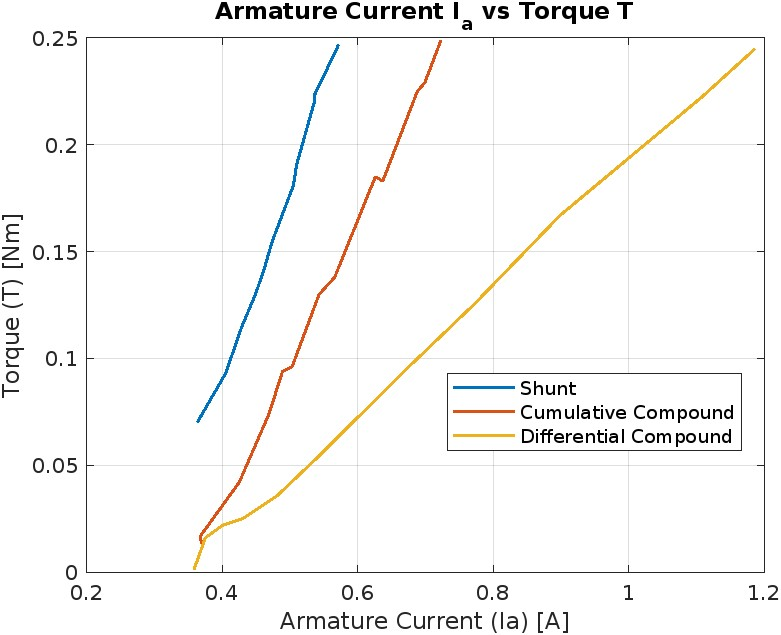
\includegraphics[width=0.85\linewidth]{Images/1.2}
			\caption{ $I_a$ vs. Torque (T) Graph }
			\vspace{0.1cm}
		\end{subfigure}
		
		\begin{subfigure}[t]{1\textwidth}
			\centering
			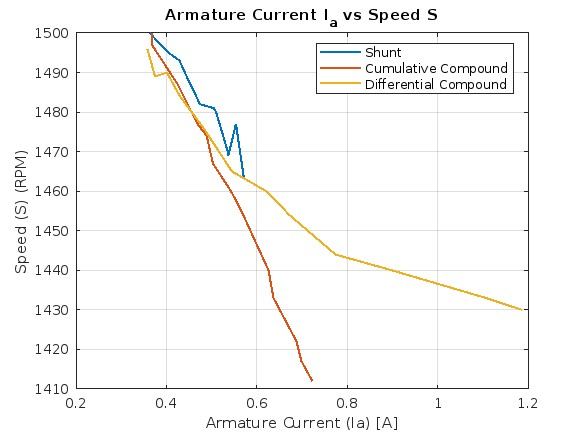
\includegraphics[width=0.95\linewidth]{Images/2.1}
			\caption{ $I_a$ vs. Speed(S) Graph}
		\end{subfigure}
		
		
	\end{figure}
	
\section{Discussion}

The experiment was conducted to investigate the Torque and Speed Characteristics of a DC Motor. The relationship between torque and speed can be described by the following equations:

\begin{equation}
	T = K I_a \Phi
\end{equation}

\[
S = \frac{V_T - I_a R_a}{K \Phi}
\]

To start the motor, it was carefully ensured that the starting resistance was kept at its maximum value, and the field resistance was also kept at its maximum. Then, the voltage of the supply was increased to 100V. After that, the starting resistance was decreased. The supply voltage was further increased to 200V, and the field resistance was then decreased to speed up the motor to 1500 rpm, the rated speed of the motor.

There were three knobs to adjust the torque value of the electrodynamometer. Initially, the torque was set to zero by adjusting the knob. Data was then recorded for the armature current, torque value, and speed at different torque levels for the DC shunt and compound motors.

	
\end{document}
